\documentclass{egee-hacked}
\usepackage{comment}
\usepackage{longtable}
\usepackage{makeidx}

\newenvironment{method}[2][]{{\vspace{4mm}\sf #2}\index{operation!
#2}\label{op:#1#2}
\par\nopagebreak\begin{tabular}{p{5mm}p{3mm}p{70mm}p{75mm}}}{\end{tabular}\\[2mm]}
\newcommand{\inpar}[2]{&$\Rightarrow$&\sf #1&#2\\}
\newcommand{\outhead}[2]{&$\Leftarrow$&\sf #1&#2\\}
\newcommand{\outpar}[2]{&&\sf #1&#2\\}
\newcommand{\faults}{}
\newcommand{\desc}{\end{tabular}\par\begin{tabular}{p{5mm}p{150mm}}
\\[-3mm] &} 
\newcommand{\OK}{
	\outhead{Tuple(1..1)}{}
	\outpar{xsd:string status}{OK}
}

\makeindex

\title{R-GMA System Specification Version}
\Version{6.2.0}
\Date{\today}
\Dissemination{PUBLIC}
% \DocumentLink{http://edms.cern.ch/document/490223/}

\Abstract{
This document presents the System Specification for the Information and 
Monitoring Services middleware component (R-GMA) in sufficient detail to 
support design verification, detailed design and test specification. It 
specifies precisely the interfaces and externally visible behaviour of all the 
R-GMA services.

The document is structured with a single chapter containing a technical
overview of the system, followed by a separate chapter for each of
the R-GMA services, with a standard set of headings in each of these chapters.
Chapters on security, SQL language support, service data types and
service parameters complete the document.}

\begin{document}

\begin{center}
% {\bf Document Change Log}
{}
\end{center}

% \begin{tabularx}{\textwidth}{|l|l|X|X|}
% \hline
% {\bf Issue } & {\bf Date  } & {\bf Comment } & {\bf Author  } \\   \hline
% 1.0 & 31 March 2005 & First release & JRA1-UK \\ 
% \hline
% 1.1 & 18 April 2006 & First release, first revision & JRA1-UK \\ 
% \hline
% \end{tabularx}
% 
% \begin{center}
% {\bf Document Change Record}
% \end{center}
% 
% \begin{tabularx}{\textwidth}{|l|X|}
% \hline {\bf Item } & {\bf Reason for Change } \\ \hline 
% 
% Updated consumer example & To avoid hanging on isExecuting() \\
% 
% Added explanation
% to allowed SQL on duplicate columns & Needed to support chunking. \\
% 
% \hline
% Added resilient consumer and producer examples & To aid users\\
% \hline
% 
% \end{tabularx}

\input{copyright}


\newpage
\tableofcontents

\newpage
\section{Introduction}
\label{sec:Introduction}

\subsection{Purpose and Structure of this Document}

This document presents the more important aspects of the design for the Information
and Monitoring Services middleware component (R-GMA) where it is not convenient
to use comments in the code. 

The various sections describe different parts of the system.

It is suggested that you read first about the Primary Producer Service
in Section \ref{sec:primaryProducerService} and then from the Request
Management Subsystem in Section \ref{sec:requestManagementSubsystem}
down to and including the Remote Call Subsystem in Section
\ref{sec:remoteCallSubsystem}.

\newpage
\section{Message Formats}\label{sec:MessageFormat}

\subsection{Data types}

An important part of these chapters is the list of operations and their input 
and output parameters. Input parameters are prefixed by $\Rightarrow$ and 
output parameters by $\Leftarrow$. Parameters may be omitted or repeated as
indicated by the notation:

\begin{description}
\item[(1..1)] Exactly once - the default
\item[(0..1)] May be omitted
\item[(1..*)] At least one
\item[(0..*)] Any number
\end{description}

after the basic type name. Types take the following values:

\begin{description}
\item[xsd:string] a sequence of Unicode characters
\item[xsd:boolean] the literals \textit{true} or \textit{false} encoded as strings
\item[xsd:int] an integer in the range $[-2^{31},2^{31} -1]$
\item[xsd:long] an integer in the range $[-2^{63},2^{63} -1]$
\item[Tuple] a tuple. This is followed by a list of the fields within the tuple.
These can be of any of the types mentioned - except for another tuple.
\end{description}

\subsection{Request}

Simple requests (such as xsd:string) values are sent as http request parameters 
(either POST or GET) and Tuples are encoded as one or more result sets within 
an XML string sent as a single http parameter. 

\subsection{Response}

The output is sent as an XML encoding of one or more R-GMA tuple sets. 

Errors are also encoded as XML.

\subsection{XML formats}

\subsubsection{Tuple set}\label{sec:TupleXML}

A single result set looks like:

\begin{verbatim}
<r m="Be warned" r="2" c="2">
  <v>Row 1 Col 1</v>
  <v>Row 1 Col 2</v>
  <n/>
  <v></v>
  <e/>
</r>
\end{verbatim}

The result set has an (optional) and has 2 rows and 2 columns as indicate by the
r and c attributes which default to 1. The data values then follow inside
\verb!<v></v>! or \verb!<n/>! to indicate the null value. The \verb!<e/>!
indicates that there is no more data.

With these rules a simple ``OK'' message is just

\begin{verbatim}
<r><v>OK</v><e/></r> 
\end{verbatim}

Multiple tuple sets must be wrapped in \verb!<s></s>! as shown below:

\begin{verbatim}
<s>
  <r><v>OK</v><e/></r> 
  <r><v>OK</v><e/></r>
</s> 
\end{verbatim}

\subsubsection{Errors}

A temporary exception is represented as:

\begin{verbatim}
<t m="This may recover" o="1"/>
\end{verbatim}

where the o attribute shows the number of succesfgul operations and defaults to
0.

A permanent exception uses p instead of t. For example:

\begin{verbatim}
<p m="This will not recover"/>
\end{verbatim}

The unknown resource message is very simple - it is just:

\begin{verbatim}
<u/>
\end{verbatim}




\newpage
\section{Primary Producer Service}\label{sec:PrimaryProducer}\index{primary producer}

\subsection{Description}

Primary Producer resources are created by the Primary Producer Service
at the request of a user who wishes to publish tuples into to one or
more tables in a virtual database\index{virtual database}.
The principal components of a
Primary Producer resource are shown in the picture below. They contain
tuple stores\index{tuple store} to hold tuples inserted by the user,
and they have an SQL query processor to run consumer queries against
their tuple stores. They are the primary source of data in a virtual
database. They all support continuous queries, and can be configured
to support any combination of latest and history queries as well.

\begin{center}
\includegraphics[width=145mm]{pp_detail}
\end{center}

The Primary Producer Service is responsible for authenticating all users and
services that connect to it, and for authorizing all operations and all requests
to access its tuple stores, as specified in chapter~\ref{sec:Security}.

\subsection{Interface}

\subsubsection{User Interface}

\begin{method}{createPrimaryProducer}
\inpar{xsd:boolean isHistory}{If history queries are supported}
\inpar{xsd:boolean isLatest}{If latest queries are supported}
\inpar{xsd:string type} {DATABASE or MEMORY}
\inpar{xsd:string logicalName}{The logical name should not be
be specified for type MEMORY. For type DATABASE it is optional.} 
\outhead{Tuple(1..1)}{}
\outpar{xsd:int connectionId}{connectionId of new Primary Producer resource.} 
\desc
Creates a new Primary Producer resource and returns its endpoint. The
Primary Producer is not added to a Registry until
\textit{declareTable} is called. The user cannot prevent Primary
Producers from supporting continuous queries, but support for latest
and/or history queries is optional. Primary Producers can use any type
of storage, regardless of the query types they support. Tuple stores can be
made permanent by providing a \textit{logical name} for the tuple store as
described in \ref{sec:PrimaryProducerTupleStores}. The termination interval is
described in \ref{sec:PrimaryProducerCreating}.
\end{method}

\begin{method}{declareTable}
\inpar{xsd:int connectionId}{Primary Producer resource identifier.}
\inpar{xsd:string tableName}{VDBTable to register.}
\inpar{xsd:string predicate}{Producer's predicate.}
\inpar{xsd:int hrpSec}{History Retention Period in seconds.}
\inpar{xsd:int lrpSec}{Latest Retention Period in seconds.}
\OK
\desc
Adds a table to the list of tables to which this producer may publish tuples,
as described in \ref{sec:PrimaryProducerDeclaring} below. The table name must
have an explicit virtual database name prefix (separated from it by a dot).
The format of the predicate is specified in \ref{sec:SQLPredicates}, and
the retention periods are described in \ref{sec:PrimaryProducerRemoving} (the 
latest retention period can be overridden in \textit{insert}). 
\end{method}

\begin{method}{insert}
\inpar{xsd:int connectionId}{Primary Producer resource identifier.}
\inpar{xsd:string insert}{SQL INSERT statement.}
\inpar{xsd:int(0..1) lrpSec}{Latest Retention Period in seconds.}
\OK
\desc
Inserts one or more tuples into a primary producer resource's tuple stores, as
described in \ref{sec:PrimaryProducerInserting}. The format of the insert
statement is specified in \ref{sec:SQLInsert}; as with \textit{declareTable},
the table name must have an explicit virtual database name prefix. Inserted
tuples must match the producer's predicate and the table schema or they will be
rejected. If the latest retention period is omitted, the default specified in
the call to \textit{declareTable} will be used. If a tuple is found to be invalid or cannot
be inserted for any reason, the operation will stop and throw an
RGMAException indicating the number of tuples successfully inserted in
its \textit{numSuccessfulOps} field (those tuples will remain in the tuple
stores).
\end{method}

\begin{method}{getLatestRetentionPeriod}
\inpar{xsd:int connectionId}{Primary Producer resource identifier.}
\inpar{xsd:string tableName}{VDBTable name.}
\outhead{Tuple(1..1)}{}
\outpar{xsd:int hrpSec}{Latest Retention Period in seconds.}
\desc Returns a Primary Producer resource's declared Latest Retention Period for
a given table.
\end{method}

See also the common producer service operations:
getHistoryRetentionperiod~\ref{op:getHistoryRetentionPeriod}.

See also the common resource management service operations:
close~\ref{op:close} and
destroy~\ref{op:destroy}.

See also the operation common to all services:
getProperty~\ref{op:getProperty}.

\subsubsection{System Interface}

See  the common producer service operations:
start~\ref{op:start} and abort~\ref{op:producerabort}.

See the common resource management service operation:
ping~\ref{op:resourceping}.

\subsection{Details}
\subsubsection{Creating and destroying Primary Producers}\label{sec:PrimaryProducerCreating}

A new Primary Producer Resource is created when a user calls the
\textit{createPrimaryProducer} operation and is destroyed when the
user calls the \textit{close} or \textit{destroy} operations. The
special processing for \textit{close} is desribed below. In addition,
if the service does not hear from the user for a period exceeding the
\textit{termination interval}\index{termination interval}, the service
will initiate a \textit{close} operation on the resource. A call to
any user operation on the resource is sufficient to keep it alive.

\subsubsection{Tuple stores}\label{sec:PrimaryProducerTupleStores}\index{tuple store}

The Primary Producer's history and latest tuple stores were described in 
\ref{sec:BackgroundTupleManagement}. They may be physically in memory or 
database storage. The memory storage may also make use of an RDBMS (typically 
memory resident) but is transient. A single producer uses 
only one type of storage for all types of queries that it supports.

The Primary and Secondary Producer services only uses stores created and 
managed by themselves. Tuple stores are normally temporary and are destroyed 
along with the producer resource, but users can make atuple store with database 
storage permanent by specifying a \textit{logical name} for the tuple store 
when they create a new Primary (or Secondary) producer. If the service is 
running in secure mode, the user's Distinguished Name (DN) is prefixed to the 
logical name. In insecure mode, the user must make the name unique within the 
service by some other means. Permanent tuple stores are not destroyed when a 
producer resource is destroyed, so they can be re-used by creating a new 
producer and naming the same store, provided there are no other producers using 
it already. The user can then re-declare any table that is already in the store 
(with a compatible predicate - see \ref{sec:SQLPredicates}) and any existing 
tuples will be automatically recovered. The names and some information about 
tuple stores can be obtained by calling \textit{listTupleStores}. Permanent tuple 
stores are deleted by calling \textit{dropTupleStore}. R-GMA only allows the 
the \textit{owners} of existing tuple stores to re-use or list them.

\subsubsection{Declaring tables}\label{sec:PrimaryProducerDeclaring}\index{declare table}

Producers must declare their intention to publish to a table by calling
\textit{declareTable} before they can insert tuples. The table definition must
already exist in the schema (see \ref{sec:SQLCreateTable}). The Primary
Producer Service obtains the table
definition from the schema by calling \textit{getFullTableDetails} and creates
the corresponding table in the resource's tuple stores (or if it already exists
in a named tuple store, checks its structure). If the
schema specifies that the table should be indexed, the producer creates the
indexes if possible, and also indexes the \textit{RgmaTimestamp} column (see
below).  It then registers the producer as a publisher for
that table, by calling the registry's \textit{registerProducerTable} operation.
The service must be ready to service consumer queries against the resource's
tuple stores as soon as this notification is sent.
This registry operation returns a list of any relevant continuous consumers
and the producer service must send an \textit{addProducer} message to each of
them to notify them about the new producer.
The producer service will also periodically re-send the
\textit{registerProducerTable} to the registry on the user's behalf, to
maintain the producer's entries in the registry throughout its lifetime. The
list of consumers returned is used to help check that consumers are still alive
(see \ref{sec:PrimaryProducerStoppingQueries}).
The user can declare more than one table in a single producer, and these can
even be in different virtual databases. All the tables are treated
independently by the producer service, except for processing ``join'' queries.

\subsubsection{Inserting tuples}\label{sec:PrimaryProducerInserting}\index{insert}

Tuples are inserted into the producer service's tuple storage by calling the
\textit{insert} or \textit{insertList} operations. They are checked for type
against the schema, and for content against the producer's declared predicate.
The following metadata is added to each tuple by the service:

\bigskip\begin{tabular}{llp{95mm}}
MeasurementDate&DATE&This and the next column will be supported for a while for
backward compatibility. At some stage they will be turned into user columns so
that they can be eliminated.\\
MeasurementTime&TIME&See above\\
RgmaTimestamp&TIMESTAMP(9)&
UTC tuple time-stamp: only added by R-GMA if not already filled in by the user;
those added by R-GMA will only have a resolution of 1ms
(see \ref{sec:SQLDataTypes} for the format of a TIMESTAMP)\\
RgmaLRT&TIMESTAMP(6)&
UTC Latest Retention Time (see below)\\
RgmaOriginalServer&VARCHAR(255)&
Hostname (including domain name) of server publishing the information.\\
RgmaOriginalClient&VARCHAR(255)&
Hostname (including domain name) of client publishing the information.\\
\end{tabular}\par\bigskip

Tuples are inserted to the tuple stores and streamed to subscribed consumers
as described in \ref{sec:BackgroundTupleManagement}. If one of the producer's
tuple stores fills up, the service temporarily blocks inserts by returning
an RGMABufferFullException until tuples expire and can be removed, as
described below.

A Producer making use of a named tuple store should avoid sending tuples that
have already been sent by another producer that used the store previously.

\subsubsection{Removing tuples}\label{sec:PrimaryProducerRemoving}\index{History Retention Period}

The user must set a \textit{History Retention Period (HRP)} and a 
\textit{Latest Retention Period (LRP)} for each declared table. The HRP is 
recorded in the registry indicating to the mediator the maximum age of tuples 
it guarantees to maintain in its history tuple store. The Primary Producer 
Service adjusts the HRP it sends to the registry to take account of the actual 
age of its history tuple store (which will be very short for a new producer), 
and updates it in the periodic calls to \textit{registerProducerTable} up to 
the value set by the user as time progresses. The LRP\index{Latest Retention 
Period} is used to calculate a \textit{Latest Retention Time 
(LRT)}\index{Latest Retention Time}\index{LRT|see{Latest Retention Time}} for 
each tuple by adding it to the tuple's RgmaTimestamp (the table-default LRP may be 
overridden in each call to \textit{insert}). The LRT is written into the 
tuple's metadata because Secondary Producers must also respect it. The two 
retention periods are independent. A history tuple store records the time of
insertion of each tuple into the tuple store and uses this to work out when the
tuples should be expired. The same rule applies to a tuple arriving in a tuple
store managed by a secondary producer.

Tuples that have expired in either tuple store can be removed by the service,
and the service is obliged to periodically clean up: it is not allowed to run
out of storage and block inserts if it could free up storage by deleting
expired tuples. In addition, tuples in the latest tuple store that have
exceeded their LRT must \textit{never} take part in latest queries.

The distinction between \textit{close}\index{close} and
\textit{destroy}\index{destroy} on a Primary Producer is that a \textit{close} 
will wait for tuples to be streamed to any continuous consumers that have not 
yet received them, and will also wait for any tuples in a memory based history 
tuple store to expire before the producer is destroyed. Note that the wait for 
tuples to expire does not apply to the latest tuple store nor to tuple stores 
using database storage. During this time, the producer will remain registered 
and still accept new history queries and latest (but not new continuous 
queries) for each declared table until all tuples for the table have expired 
from the history tuple store, at which point the corresponding table is 
unregistered, by calling \textit{unregisterProducerTable}. When all tables have 
been unregistered and all tuples have been streamed, the producer resource is 
destroyed.

\subsubsection{Processing queries}\label{sec:PrimaryProducerQueryProcessing}

Consumer services send a \textit{start} message to a Primary Producer
to request it to execute a query and start streaming the resulting
tuples back to the consumer service. Continuous queries receive all old tuples
available in the producer's history store since the start time specified in the
\textit{start} call, followed by all new tuples as they are inserted to the
producer. One-time queries execute on the current
contents of the history and latest tuple stores only and terminate when they've
returned all of the results to the consumer service.

The streaming protocol and the streaming server in the consumer service are
described in section \ref{sec:ConsumerStreaming}. As described there, tuples
are streamed in \textit{chunks}, with the last chunk for a one-time query
distinguished by an \textit{end-of-results} flag.
The connection details of the streaming server, and the maximum
number of tuples it will accept in a single chunk, are passed in the
\textit{start} call. It is the responsibility of the implementation to ensure
that the results of a one-time query are evaluated just once and are immune to
changes to the tuple stores while the results are being streamed.

\subsubsection{Stopping queries}\label{sec:PrimaryProducerStoppingQueries}

One-time queries automatically terminate when the last tuple has been
streamed to the consumer. All queries may be terminated by running
for longer than the query \textit{timeout} specified in the call to
\textit{start}.

\newpage
\section{Secondary Producer Service}\label{sec:SecondaryProducer}\index{secondary producer}

\subsection{Description}

Secondary Producer resources are created by the Secondary Producer
Service at the request of a user to
\textit{republish}\index{republish} one or more tables in a virtual
database. Republishing means running a ``SELECT * WHERE'' query
against a table in the virtual database and publishing the resulting
tuples back to the same table. The mediator ensures this isn't
recursive. As the picture below shows, the principal components of a
Secondary Producer are the same as a Primary Producer. All Secondary
Producers support continuous queries, and can be configured to support
any combination of latest and history queries as well.

\begin{center}
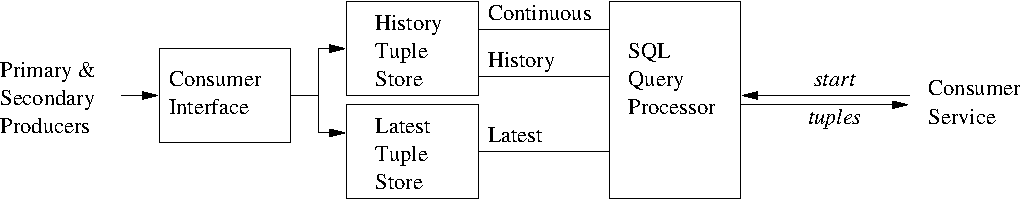
\includegraphics[width=160mm]{sp_detail}
\end{center}

The value of a Secondary Producer is that it creates real tables from
virtual ones, because it collects all tuples inserted into the virtual database
for any table it's republishing, into its own tuple stores. This means it can
act as an archiver for the tables, can answer queries involving joins between
them (even tables in different VDBs) because they're all in one database,
and can be used to reduce the load on other producers.

The Secondary Producer Service is responsible for authenticating all
users and services that connect to it, and for authorizing all
operations and all requests to access its tuple stores, as specified
in chapter \ref{sec:Security}.

\subsection{Interface}

\subsubsection{User Interface}

\begin{method}{createSecondaryProducer}
\inpar{xsd:boolean isHistory}{If history queries are supported}
\inpar{xsd:boolean isLatest}{If latest queries are supported}
\inpar{xsd:string type} {DATABASE or MEMORY}
\inpar{xsd:string logicalName}{The logical name should not be
be specified for type MEMORY. For type DATABASE it is optional.} 
\outhead{Tuple(1..1)}{}
\outpar{xsd:int connectionId}{connectionId of new Secondary Producer resource.} 
\desc Creates a new Secondary Producer resource and returns its endpoint. The
Secondary Producer is not added to a Registry until \textit{declareTable} is
called. The user cannot prevent Secondary Producers from supporting
continuous queries, but support for latest and/or history queries is optional.
Secondary Producers can use any type of storage, regardless of the query types
they support. Tuple stores can be made permanent by providing a
\textit{logical name} for the tuple store as described in
\ref{sec:SecondaryProducerTupleStores}.
The termination interval is described in \ref{sec:SecondaryProducerCreating}.
\end{method}

\begin{method}{declareTable}
\inpar{xsd:int connectionId}{Secondary Producer resource identifier.}
\inpar{xsd:string tableName}{VDBTable to register.}
\inpar{xsd:string predicate}{Producer's predicate.}
\inpar{xsd:int hrpSec}{History Retention Period in seconds.}
\OK
\desc
Adds a table to the list of tables republished by this producer, as described
in \ref{sec:SecondaryProducerDeclaring}. The table name must have an explicit
virtual database name prefix (separated from it by a dot).
The format of the
predicate is specified in \ref{sec:SQLPredicates}; by construction, a Secondary
Producer will republish \textit{all} tuples that match its predicate. The
retention period is described in \ref{sec:SecondaryProducerRemoving}.\\
\end{method}\par

\begin{method}{showSignOfLife}
\inpar{xsd:int connectionId}{Resource identifier.}
\OK
\desc Sends a sign-of-life request to a resource as a way to keep
the resource alive. Any other user operation on the resource will also serve
to keep it alive.
\end{method}

See also the common producer service operations:
getHistoryRetentionperiod~\ref{op:getHistoryRetentionPeriod}.

See also the common resource management service operations:
close~\ref{op:close} and destroy~\ref{op:destroy}.

See also the operations common to all services:
getProperty~\ref{op:getProperty}.

\subsubsection{System Interface}

\begin{method}{secondary}{addProducer}
\inpar{xsd:int connectionId}{Consumer resource identifier.}
\inpar{xsd:string url}{Producer URL.}
\inpar{xsd:int id}{Producer resource identifier.}
\inpar{xsd:string tableName}{Table name}
\inpar{xsd:string predicate}{Predicate}
\inpar{xsd:int hrpSec}{History Retention Period in seconds}
\inpar{xsd:boolean isHistory} {If producer supports history queries}
\inpar{xsd:boolean isLatest}{If producer supports latest queries}
\inpar{xsd:boolean isContinuous}{If producer supports continuous queries}
\inpar{xsd:boolean isStatic}{If producer supports static queries}
\inpar{xsd:boolean isSecondaryProducer}{If producer is secondary}
\inpar{xsd:string qosAttrib}{The QOS attribute - not used currently}
\OK
\desc Sent by a producer service to a continuous consumer or secondary producer
to notify it about an
addition to the list of relevant producers in the registry. Ignored if the
query is not currently executing. See the \textit{plan maintenance} section
(\ref{sec:ConsumerPlanMaintenance}) for how the consumer or secondary
producer should react to this.
\end{method}

\begin{method}{removeProducer}
\inpar{xsd:int connectionId}{Consumer resource identifier.}
\inpar{xsd:string url}{Producer URL.}
\inpar{xsd:int id}{Producer resource identifier.}
\OK
\end{method}

See  the common producer service operations:
start~\ref{op:start} and abort~\ref{op:producerabort}.

See the common resource management service operation:
ping~\ref{op:resourceping}.

\subsection{Details}
\subsubsection{Creating and destroying Secondary Producers}\label{sec:SecondaryProducerCreating}

A new Secondary Producer resource is created when a user calls the
\textit{createSecondaryProducer} operation and is destroyed when the user calls
the \textit{close} or \textit{destroy} operations. In addition,
if the service does not hear from the user for a period exceeding the
\textit{termination interval}, the service will initiate a \textit{close} operation
on the resource. A call to any user operation on the resource is sufficient
to keep it alive.

\subsubsection{Tuple stores}\label{sec:SecondaryProducerTupleStores}

These are exactly as in the Primary Producer Service (see
\ref{sec:PrimaryProducerTupleStores}) but System Administrators should
be even more wary of granting direct access to permanent tuple stores
maintained by Secondary Producers because Secondary Producers are granted
special access to the tuple stores of the producers from which they are
consuming, and those producers trust them to enforce the data access rules
of the VDB when republishing the data.

\subsubsection{Declaring tables (as a producer)}\label{sec:SecondaryProducerDeclaring}

The semantics of \textit{declareTable} are identical from the user's point of 
view to the Primary Producer, except that there is no Latest Retention Period 
to set. Internally, the service prepares the tuple stores then registers the 
Secondary Producer resource as a producer by calling 
\textit{registerProducerTable} and periodically calls this again to keep itself 
registered.

\subsubsection{Declaring tables (as a consumer)}\label{sec:ConsumerDeclaring}

Unlike a Primary Producer, the Secondary Producer must also act as a continuous
consumer for each declared table, by running a 
``SELECT * FROM \textit{tableName} WHERE \textit{predicate}'' query on the
virtual database. The procedure for identifying and notifying the producers
that will answer this query is exactly as in \ref{sec:ConsumerStarting} and
the list of producers is maintained as described in
\ref{sec:ConsumerPlanMaintenance}. A side effect of this is to register the
Secondary Producer resource as a \textit{secondary} consumer and keep it
registered. Flagging the resource as a secondary consumer simply allows
the mediator to ensure that it doesn't generate recursive query plans - in all
other respects, the mediator and the registry service treat the secondary
producer resource like any other continuous consumer and no further distinction
is made in this document. Likewise, the secondary producer presents the same
streaming interface to producers as described in
\ref{sec:ConsumerStreaming} for continuous consumers.

\subsubsection{Inserting tuples}\label{sec:SecondaryProducerInserting}
Tuples are inserted into a Secondary Producer by the service itself (by its 
streaming server). Users do not insert tuples into a Secondary Producer 
directly. Secondary Producers do not modify the tuples they store in any way.

\subsubsection{Removing tuples}\label{sec:SecondaryProducerRemoving}
The rules for History Retention Periods and Latest Retention Times in a
secondary producer are identical to a primary producer.

The \textit{close} call, however, is different from a primary producer. Since a
secondary producer must stop consuming immediately after a \textit{close}
request it must also stop servicing queries too, because it no longer holds a
complete set of tuples for the tables that it claims to republish.
Therefore \textit{close} means the same as \textit{destroy} in a secondary
producer.

\subsubsection{Processing queries}\label{sec:SecondaryProducerQueryProcessing}

Query processing in a Secondary Producer is identical to a Primary Producer
(see \ref{sec:PrimaryProducerQueryProcessing}).

\subsubsection{Stopping queries}\label{sec:SecondaryProducerStoppingQueries}

This is also identical to a Primary Producer
(see \ref{sec:PrimaryProducerStoppingQueries}).



\newpage
\section{On-demand Producer Service}\label{sec:OnDemandProducer}\index{on demand producer}
\subsection{Description}

On-demand Producer resources are created by the On-demand Producer Service
at the request of a user who wishes to make an external data store available
through a virtual database. They are registered in the same way as the other
producer types and their queries are parsed, validated and authorized like
queries to the other producer types, but they only support static queries,
are not used by Secondary Producers, have no internal tuple storage, and
have no concept of retention periods. As the picture below shows, queries are
simply handed off to a user-defined application (\textit{query handler}) that
is expected to process the query and return the resulting tuples on demand.

\begin{center}
\includegraphics[width=110mm]{odp_detail}
\end{center}

The On-demand Producer Service is responsible for authenticating all users and
services that connect to it and for authorizing all operations and requests to
access its users' external data stores, as specified in chapter
\ref{sec:Security}.

\subsection{Interface}

\subsubsection{User Interface}

\begin{method}{createOnDemandProducer}
\inpar{xsd:string hostName}{Hostname of machine to which to connect to get data
to answer queries.}
\inpar{xsd:int port}{Port to which to connect to get data
to answer queries.}
\outhead{Tuple(1..1)}{}
\outpar{xsd:int connectionId}{connectionId of new On-demand Producer resource.} 
\desc
Creates a new On-demand Producer resource and returns its endpoint. The
On-demand Producer is not added to a Registry until \textit{declareTable} is
called. On-demand producers have no tuple stores and only support static
queries.
\end{method}


\begin{method}{declareTable}
\inpar{xsd:int connectionId}{On-demand Producer resource identifier.}
\inpar{xsd:string tableName}{VDBTable to register.}
\inpar{xsd:string predicate}{Producer's predicate.}
\OK
\desc
Adds a table to the list of tables for which this producer will return tuples,
as described in \ref{sec:OnDemandProducerDeclaring}.
The table name must have an explicit virtual database name prefix (separated
from it by a dot). The format of the predicate is specified
in \ref{sec:SQLPredicates}; all returned tuples must match this predicate or
they will be rejected by the producer. 
\end{method}

See also the common producer service operations:
getHistoryRetentionperiod~\ref{op:getHistoryRetentionPeriod}.

See also the common resource management service operations:
close~\ref{op:close} and
destroy~\ref{op:destroy}.

See also the operations common to all services:
getProperty~\ref{op:getProperty}.

\subsubsection{System Interface}

See  the common producer service operations:
start~\ref{op:start} and abort~\ref{op:producerabort}.

See the common resource management service operation:
ping~\ref{op:resourceping}.

\subsection{Details}
\subsubsection{Creating and destroying On-demand Producers}\label{sec:OnDemandProducerCreating}

A new on-demand producer resource is created when a user calls the
\textit{createOnDemandProducer} operation and is destroyed when the
user calls the \textit{close} or \textit{destroy} operations. In
addition, if the service does not hear from the user for a period
exceeding the \textit{termination interval}, the service will initiate
a \textit{close} operation on the resource. A call to any user
operation on the resource is sufficient to keep it alive.

\subsubsection{The query handler}

The on-demand producer connects to the specifed hostname and port via an SSL
socket connection to answer user queries. R-GMA
expects the query handler application to be listening for queries
throughout the lifetime of the on-demand producer resource.

\subsubsection{Declaring tables}\label{sec:OnDemandProducerDeclaring}

On-demand producers must register any tables for which they will
answer queries by calling \textit{declareTable}. The On-demand
Producer Service registers the producer as a publisher for that table
by calling the registry's \textit{registerProducerTable} operation and
will periodically re-send the \textit{registerProducerTable} to the
registry on the user's behalf, to maintain the producer's entries in
the registry throughout its lifetime. The user can declare more than
one table in a single producer, and these can even be in different
virtual databases. Whether or not ``join'' queries can be processed
depends only on the capabilities of the query handler that answers the
producer's queries.

\subsubsection{Processing Queries}\label{sec:OnDemandProducerQueryProcessing}

Consumer Services send a \textit{start} message to an On-demand
Producer to request it to execute a query and start streaming the
resulting tuples back to the consumer service. The query is forwarded
to the registered query handler for processing (see below for the protocol),
and the tuples (if any)
returned by the query handler are streamed by the On-demand Producer service
back to the consumer's streaming server, exactly as in a one-time query to
any other type of producer (see \ref{sec:ConsumerStreaming}). A query may be
stopped by the consumer service by calling \textit{abort}. Queries
will also be automatically aborted by the On-demand Producer Service
if they run for more than the \textit{timeout} specified in the call
to \textit{start}.

The On-demand producer service will append the standard metadata columns
(see \ref{sec:PrimaryProducerInserting}) to each tuple for
consistency with the table definition in the schema, before streaming
them back to the consumer service, but the columns will all be populated
with NULLs.

See section
\ref{sec:SQLCharacterSets} for information about the character sets used in
R-GMA (this will affect both the SQL query sent to the query handler, and its
response).

\subsubsection{Query handler protocol}

The On-demand Producer service contacts the query handler by opening a TCP
connection on the host
and port specified in the URI and writing the SQL SELECT query and the maximum
number of tuples it will allow in a result set, to the port. The two parameters
are separated by a semi-colon and the request is terminated by a CR-NL end of 
line marker. The query handler must respond by sending a series of result sets
(chunks) each containing no more than the requested number of tuples, or it must
return an exception. The query handler should mark the end of the response by
shutting the TCP connection.

The result sets and exceptions returned by the query handler are XML fragments,
each containing a single XMLResultSet or XMLException. The XMLResultSet looks
like this:

\begin{verbatim}
<?xml version="1.0" encoding="UTF-8" standalone="no"?>
  <XMLResultSet endOfResults="true">
    <columnMetaData>
      <name>column-name</name>
      <type>NNN</type>
      <table>table-name</table>
    </columnMetaData>
    <row>
      <col>column-value</col>
      <col isNull="true"/>
    </row>
  </XMLResultSet>
\end{verbatim}
                                                                                
where \textit{columnMetaData} and \textit{col} are repeated for each
column, and \textit{row} is repeated for each row. The valid values
for \textit{type} are 4 (INTEGER), 7 (REAL), 8 (DOUBLE PRECISION), 91
(DATE), 92 (TIME), 93 (TIMESTAMP), 1 (CHAR) and 12 (VARCHAR). The
\textit{endOfResults} and \textit{isNull} flags both default to \textit{false} if
omitted. The \textit{XMLResultSet} element is allowed to be entirely
empty.  The last result set must contain an \textit{endOfResults} flag
set to \textit{true} (even if it is empty).

The XMLException looks like this:

\begin{verbatim}
<?xml version="1.0" encoding="UTF-8" standalone="no"?>
  <XMLException>
    <message>message-string</message>
  <XMLException>
\end{verbatim}

The On-demand producer service will shut the TCP connection if the query
handler exceeds the tuple limit in a single result set (chunk), or
it receives an \textit{abort} request, or if some other error occurs. The
query handler must ensure that the result of a query does not change during
the time it takes to deliver all of the tuples to the on-demand producer
service.

\subsection{Error Handling}

The default handling for all errors is to stop processing, make the resource
stable if possible and notify the user
(see section \ref{sec:BackgroundErrorReporting}).

\newpage
\section{Producer Operations}\label{sec:Producer}\index{producer}

Operations defined here are are common to all producers. 

\subsection{Interface}

\subsubsection{User Interface}

\begin{method}{getHistoryRetentionPeriod}
\inpar{xsd:int connectionId}{Producer resource identifier.}
\inpar{xsd:string tableName}{VDBTable name.}
\outhead{Tuple(1..1)}{}
\outpar{xsd:int hrpSec}{History Retention Period in seconds.}
\desc Returns a Producer resource's declared History Retention Period for
a given table.
\end{method}

\subsubsection{System Interface}

\begin{method}{start}
\inpar{xsd:int connectionId}{Producer resource identifier.}
\inpar{xsd:string select}{Consumer's SQL SELECT query.}
\inpar{xsd:string queryType}{``continuous", ``latest", ``history" or ``static"}
\inpar{xsd:int(0..1) timeIntervalSec}{Time interval associated with queryType}
\inpar{xsd:long timeoutSec}{Query timeout in seconds.}
\inpar{xsd:string consumerURL}{Consumer's URL.}
\inpar{xsd:int consumerId}{Consumer's resource ID.}
\inpar{xsd:string streamingURL} {URL for streaming.}
\inpar{xsd:int streamingPort} {Port number for streaming.}
\inpar{xsd:int bufferSize} {Maximum buffer size to use for streaming.}
\inpar{xsd:int streamingProtocol} {Protocol number to use for streaming.}
\inpar{xsd:string qosAttrib}{Consumer's desired Quality of Service.}
\outhead{Tuple(1:1)}{}
\outpar{xsd:string tableName}{}
\outpar{xsd:long timestamp}{}
\desc Requests the producer to execute a query and start 
streaming tuples to the specified consumer. The query will have been generated 
by the mediator and can be assumed to be valid: both tables and views may be 
queried (see~\ref{sec:SecurityViews}). It is assumed that there is a streaming 
server listening on the given endpoint, ready to receive the tuples pushed to 
it.
\end{method}

\begin{method}[producer]{abort}
\inpar{xsd:int connectionId}{Producer resource identifier.}
\inpar{xsd:string consumerURL}{Consumer's URL.}
\inpar{xsd:int consumerId}{Consumer's resource ID.}
\OK
\desc Requests the producer to stop streaming tuples to the specified consumer and
abort the query.
\end{method}
\newpage
\section{Consuming Information}

\label{sec:consumer}

\subsection{Types of Query}
There are four types of query: \emph{continuous}, \emph{latest}, {\sl
history} and \emph{static} (the latter is only supported by on-demand
producers). The set of queries that a particular producer supports is
recorded in the registry. All query types except static can take an
optional time interval parameter (see below).

A continuous query causes all new tuples that match the query, to be
streamed into the consumer's tuple-storage as soon as they are
inserted into the virtual table by the producers. Streaming continues
until the consumer requests it to stop. If a time interval is
specified, the consumer will additionally receive any tuples which are
already in the virtual table when the query starts, and which are no
older than the time interval. There is no guarantee that tuples are
time-ordered. All primary and secondary producers support continuous
queries. On-demand producers do not.

Latest and history queries are \emph{one-time} queries: they execute
on the current contents of the virtual table, then terminate. In a
history query, all versions of any matching tuples are returned; in a
latest query, only those representing the ``current state''
(see~\ref{sec:consumers}) are returned. In both cases, a time interval
may be specified with the query, to limit the age of the tuples
returned. Primary and secondary producers may optionally support
one-time queries. On-demand producers do not.

\subsection{Consumer Examples}
This provides  examples of code you might use or adapt.
\subsubsection{Simple Consumer Example}

\newpage
\section{Resource Management Operations}\label{sec:Resource}\index{resource 
management operations}

Operations defined here are are common to all resource management operations - i.e.
producers and consumers.

\subsection{Interface}

\subsubsection{User Interface}

\begin{method}{close}
\inpar{xsd:int connectionId}{Resource identifier.}
\OK
\desc Schedules a resource for destruction after the resource has completed its work.
\end{method}

\begin{method}{destroy}
\inpar{xsd:int connectionId}{Primary Producer resource identifier.}
\OK
\desc 
Destroys a Primary Producer without any special \textit{close} processing.
\end{method}


\subsubsection{System Interface}

\begin{method}[resource]{ping}
\inpar{xsd:int connectionId}{Resource identifier.}
\OK
\desc
Checks if a resource is still alive (and throws an exception if it is not).
Has no side-effects on the resource. 
\end{method}

\newpage
\section{Registry Service}
\label{sec:registryService}
\index{Service!Registry}

Package: \texttt{org.glite.rgma.server.services.registry}

The registry service has a registry instance for each VDB hosted
locally and a RemoteRegistry singleton to deal with forwarding
requests to remote registry services. Each instance is responsible for
dealing with its own replication and makes use of a RegistryDataBase
interface. An implementation of this interface is needed for each
supported RDBMS.



\subsection{Registry Instance}
\label{sec:registryInstance}

The principal components of the Registry Instance are shown in the picture at the
start of this chapter. When the instance is created, it creates a new instance of
a Registry Database and creates and starts a new Registry Cleanup and Replication
thread.  The instance has a status (\texttt{OFFLINE}/\texttt{ONLINE}) set to
\texttt{OFFLINE} when it is created. The registry instance is set to
\texttt{ONLINE} when the initialisation is complete.

All operations other than those associated with replication  have the same
signature as those in the Registry Service except that the vdbName is omitted.
The first part of all operations is to check the caller is authorized to call
this operation.

\subsubsection{Registry Replication}
\label{sec:registryReplication}
\label{sec:replicationIntroduction}
The Registry Instance is updated either by direct calls or upon
receipt of replication messages. A registry ``owns'' those records
that were last changed by direct calls and is responsible for pushing
updates of these records to other registries within the same
VDB. Records have an \texttt{isMaster} flag that \texttt{isMaster}
flag is set by any direct add request
(\texttt{getMatchingProducersForTables} or
\texttt{registerProducerTable}) and is cleared by a replication
message.

Records have a \texttt{lastContactTimeSec} which controls the purging
of old records however it is also used to detect a delayed replication
message. This is set by the registry receiving a direct call and is
subsequently replicated as part of the record.

Direct change requests are always respected, whereas replicated change
requests are ignored if they are out of date (i.e. before the
\texttt{lastContactTimeSec} associated with the record). 

If a registry should be unavailable then direct update requests will
get routed to a different registry instance and records in the new
registry will get the \texttt{isMaster flag} set. The original
registry will initially be unaware that another registry has
mastership of that record. When it receives replication messages from
the new master the \texttt{isMaster flag} will  be cleared.

The algorithm may result in more than one registry thinking that it is
master - however this is not a problem. It also possible to have no
master as the master may go down. However in all cases the system will
clean up when a registry assumes mastership for the record and
replicates its records.

If the clock on a registry is running too far behind time its
replication messages will be ignored if the receiving registry already
has an entry. If the clock is running fast then the replication
message will be received and the \texttt{lastContactTimeSec} will be
set in the future which will delay the purging of this record if it is
not explicitly deleted. This may result in non-existent resources
being returned by the registry.

Each \texttt{VDB} registry instance should log if the
\texttt{lastContactTimeSec} for a record is ahead of the current
time.

Note that where registry entries don't already exist, updates are
treated as inserts by the Registry Database and deletions of entries
that no longer exist are handled silently.

\paragraph{Full updates}

The algorithm described above assumes that all replication messages
are transmitted and processed correctly. Time stamps are associated
with the replication messages so that if a message has been lost the
recipient will know when the message is received. In this case a full
update is transmitted. This is generated by asking the Registry
Database for all records with the \texttt{isMaster} flag set.

\paragraph{The RegistryReplicationTable}

A hash table is used to hold the addRegistration and
deleteRegistration requests keyed on the primary key of the resource
entry. This means that if several addRegistration requests are
followed by a deleteRegistration request only the delete will be held.

When a request for a resource registration or deletion is received by
the Registry Instance, then in addition to passing the request to the
Registry Database it is inserted in the hash table.

When the Registry Instance replicate() operation is requested by the
Registry Cleanup and Replication a new hash table is created to take
new entries and the old one can be processed. This should be achieved
by a synchronisation lock between the call which adds to the hash
table and the code which switches the references.

A message is created from the hash table to be sent asynchronously to
all replicas using the \texttt{addReplica} call. If at the beginning
of the next cycle any messages have not been sent they are purged and
a full update will be sent instead to those replicas.

If the registry is restarted it will lose its hash table. When it
starts it must send a full update to all replicas. If the registry has
been down for some time other registries will have taken mastership
and most records will be ignored as they will be too old.

\paragraph{The addReplica message}

The addReplica message contains UTC timestamps of the last replication
cycle for this instance (\texttt{lastReplicationTime}) and the current
one (\texttt{currentReplicationTime}). This allows the recipient to
recognise if it has missed a message and to request a full update.

For a full update the \texttt{lastReplicationTime} is set to 0 so that the 
recipient will accept the message as the latest.

This is followed by an add section containing entries to add and a
delete section with keys to be deleted.

\subsubsection{Replication Operations}
This code is intended to create an \texttt{addReplicaMessage} or
\texttt{fullUpdateAddReplicaMessage} only when needed. If a remote
registry is down for a while repeated attempts will be made to send it
an \texttt{addReplicaMessage}. Once it comes back and receives a
message it will respond with \texttt{RGMAReplicaUpdateException} and
next time will get a \texttt{fullUpdateAddReplicaMessage}.

Note that the replicate call has a boolean flag \texttt{full} which is
set on the first call to request a full update.

Note also that when an \texttt{addReplica()} call is sent it is sent
asynchronously to another replica of this VDB. It does not use the
normal remote call mechanism via the \texttt{RemoteRegistry} object
but sends directly to the specified replica.



\subsection{Registry Database}

The RegistryDatabase is an interface to implementations for different
vendor specific databases with all of the SQL needed to read and
update it. The implementations uses vendor specific connection
wrappers in org.glite.rgma.server.services.registry. The database
table definitions and the methods in this component are described
here.


\subsection{RemoteRegistry}
\label{sec:RemoteRegistry}
\index{Class!RemoteRegistry}

This is the API used to forward calls to another Registry Service. It
has exactly the same interface as Registry Service but makes no use of
the authz context..  It uses the Remote Call Subsystem described in
section~\ref{sec:remoteCallSubsystem}. 

Each VDB which is not supported locally has a current registry service defined
to which calls will be forwarded. If the current registry is not defined all
services are pinged in parallel and the first to reply is selected as the
current registry. If it turns out that the current registry is set but not
reachable the current registry is cleared and a new one is sought.
\newpage
\section{Schema Service}
\label{sec:schemaService}
\index{Service!Schema}

Package: \texttt{org.glite.rgma.server.services.schema}

The SchemaService inherits from Service and owns a set of Schema
Instances. Each instance holds the schema for a single VDB. 

If an R-GMA server supports a VDB then it must offer a schema instance for that
VDB. For each VDB one instance is the master and this is controlled by a
configuration file.

All schema updates are made first to the master and then an update is requested
from the master. Other slaves are responsible for getting updates from
the master.

Each Schema Instance creates an instance of Schema Database to contact
the underlying RDBMS. Different Schema Database implementations will be
written - each peculiar to a single RDBMS to make effective use of
that system. Each schema instance has its own replication thread.

Most operations are passed to the schema instance corresponding to the
VDB name except for those which may modify the state of the
instance. These calls are all passed via the RemoteSchema to the
master schema - where they are then processed locally.  Before passing
the call on to the RemoteSchema the canForward flag must be
checked. If the flag is not true an error must be returned. All calls
to the Remote Service must have canForward set to false.

The schema instance does very little - most of the work is done by the
Schema Database which it creates when it starts.

\subsection{Schema Replication}
\label{sec:schemaReplication}
Slaves poll the master to receive updates. The master does not know
the slaves and does not hold any queues. The slaves ask for changes
since a certain time and if they don't get a reply keep asking the
same question on each replication loop. Eventually a reply will be
received and the time stamp from the master is stored. Subsequent
requests will ask for updates since the new time. To allow the master
to respond correctly, major items in the schema (Table, View and
Index) have a time stamp associated with them. This time stamp is set
when the tuple is added or updated. Child tuples, such as the columns
of a table have implicitly the same stamp. This means that if a column
is removed from a table, the table and all its remaining columns will
be transmitted upon request.

Note that when a Table, View or Index is dropped from the schema, a
time-stamped skeleton is left behind which will then have no related
columns. This makes transmitting updates very easy at the cost of a
few entries in the database. Evidently a table, view or index with no
columns should normally be treated as not present - except in
replication operations.

\subsection{Schema Database}

The SchemaDatabase is an interface to implementations for different
vendor specific databases with all of the SQL needed to read and
update it. The implementations uses vendor specific connection
wrappers in org.glite.rgma.server.services.schema. 



\newpage
\section{Service Operations}\label{sec:Service}\index{service operations}

Operations defined here are are common to all services.

\subsection{Interface}

\subsubsection{User Interface}

\begin{method}{getProperty}
\inpar{xsd:string name}{Property name.}
\inpar{xsd:string(0..1) parameter }{Property parameter.}
\outhead{xml:Any}{Property value.}
\desc Returns the current value of the requested service property. The appropriate
contents of \textit{parameter} depend on the property name. The list of
service properties is extensible and subject to change without warning.
\end{method}

\subsubsection{System Interface}

\newpage
\section{RGMAService Operations}\label{sec:Producer}\index{producer}

The RGMAService is for functions not directly related to producers, consumers,
registry or schema.

\subsection{Interface}

\subsubsection{User Interface}

\begin{method}{listTupleStores}
\outhead{Tuple(0..*)}{}
\outpar{xsd:string logicalName}{Logical name of tuple store.}
\outpar{xsd:boolean isHistory}{If logical name is associated with a history store.} 
\outpar{xsd:boolean isLatest}{If logical name is associated with a latest store.}
\desc Returns a list of all of the permanent tuple stores. A logical name may be associated with both history and latest 
stores. Only the user's own tuple 
stores are listed.
\end{method}

\begin{method}{dropTupleStore}
\inpar{xsd:string logicalName}{Logical name of tuple store.}
\OK
\desc Permanently deletes a permanent tuple store, provided it is not currently being
used by a producer. Only the user's
own tuple stores can be dropped.
\end{method}

\begin{method}{getVersion}
\outhead{Tuple}{}
\outpar{xsd:string version}{Service version.}
\desc Returns the version number of the services.
\end{method}

\begin{method}{getTerminationInterval}
\outhead{Tuple)}{}
\outpar{xsd:int terminationIntervalSec}{Termination interval in seconds.}
\desc Returns the current termination interval defined by the services.
\end{method}

\newpage
\section{Security}\label{sec:Security}\index{security}

\subsection{Introduction}

In a secure installation, R-GMA services are responsible for ensuring
the integrity and confidentiality of the virtual databases and all
user data held within the service infrastructure.  This chapter
specifies the security mechanisms used by the services to meet this
responsibility. Sites can opt to run their services with these
security mechanisms turned off, but other R-GMA services running
securely will not communicate with them.

\subsection{Risks to services and data}

The integrity of a virtual database is compromised if a person
maliciously modifies data or causes operations to execute incorrectly
so that the virtual database reaches an invalid state or returns
invalid results. This can be achieved either by direct attacks on the
service infrastructure or by abusing the operations provided by
services.

The integrity and confidentiality of user data are compromised if a
person can read or modify the data without the owner's consent. User
data in R-GMA does not just include tuples, but also query strings
(because predicates may contain user data), resource connection
details (because these could be used to launch attacks), user
identification details stored for security purposes and user names and
passwords for external data stores.  Data integrity and
confidentiality can be compromised by a malicious person making direct
attacks on the service infrastructure or abusing the operations
provided by services. They can also be compromised by the failure of a
service implementation to properly enforce data access rules.

\subsection{Securing services and data}

The service infrastructure consists of the underlying operating
system, the servlet container, external
storage used by the services (e.g. databases, configuration files, log
files), connections between services and external storage (e.g. JDBC
links), and network connections to services. With the exception of the
network connections, it is beyond the scope of this specification to
say how these can be made secure, but it is mandatory for all R-GMA
service implementations to address the security of each of these
components.

How R-GMA services secure network transfers against interception and
modification, how they control connections to services and how they
control execute access to operations and read and write access to data
stores, are all covered in the remainder of this chapter.

\subsection{Securing network transers}

All user-to-service and service-to-service connections (including
streaming) in a secure R-GMA installation use SSL to encrypt the data
as it travels over the network. Data is \textit{not} encrypted by
R-GMA within its services. If users don't trust the security of
R-GMA's services, they must encrypt the data themselves before sending
it to R-GMA.
                                                                               

\subsection{Authentication}\index{authentication}

R-GMA services must immediately terminate a user's or other service's
attempt to connect to them if their identity cannot be
authenticated. If a user chooses to use one of the R-GMA APIs, the API
will likewise abandon a connection immediately if it cannot
authenticate the service to which it is connecting (this is
\textit{mutual authentication}). The APIs return an appropriate
RGMASecurityException in response to authentication failures.

Mutual authentication is based on an exchange of encrypted messages.
Each party's identity is proved by their possession of a private key
corresponding to the public key embedded in a digital certificate
signed by a certificate authority recognised by the other party.  Currently
R-GMA services accept only X509 format certificates (including proxy certificates generated by
grid-proxy-init or voms-proxy-init).

The mechanism used for authentication and for managing Certificate
Authority (CA) certificates and their supporting files (revocation
lists, signing policies, etc) is implementation-dependent.

\subsection{Authorization}\index{authorization}

\subsubsection{Credentials}\index{credentials}

R-GMA services permit or deny access to resources (in the general
sense) to a user or another service, on the basis of
\textit{credentials} held by that user or service. Credentials are
extracted from the certificate used for authentication in some
implementation-defined way. Each credential has a name such as the
{Distinguished Name} (DN) credential found in all
certificates\footnote{The DN of host certificates contains the host
name.}.  The credentials found in the \textit{VOMS proxy certificates}
used by all EGEE services are:

\begin{itemize}
\item Membership of virtual organizations (VO);
\item Membership of groups within a virtual organization (GROUP);
\item Roles held within a virtual organization (ROLE);
\end{itemize}

and some, such as GROUP, may take more than one value.  All
authorization rules are defined in terms of combinations of zero or
more credentials, and whilst R-GMA service implementations are obliged
to support VOMS credentials, they will actually work with any type of
credential.

\subsubsection{Ownership}\index{ownership}

The servers on which R-GMA services run are owned by individual
sites\index{site}, so it is they who decide whether or not to run the
services. 

Each virtual database has an owner (typically a VO) and registry 
instances and the master schema are hosted by sites by mutual agreement with the
virtual database owner. The virtual database owner owns the registry and schema instances and
decides who can read or modify them, but they have to trust the individual
sites to implement their policy, and the sites retain overall control.

Virtual database owners control who can create, read or modify information
the schema and who can read tuples from their virtual database and who can
publish tuples to it, because they own the schema and the data access rules are
defined there. Anybody permitted to write to a table defintion in the
schema can also control who can read or write to that table within the virtual
database.

\subsubsection{Authorization points}

Access to the tuples in the tuple stores is authorized using \textit{read} and 
\textit{write} rules set for each table and view in the schema. The rule-based 
mechanisms are described below.

Access to the schema information is controlled by rules stored as part of the
VDB in addition to rules stored with a table defintion in the schema.

\subsubsection{Restricting access to columns (views)}\label{sec:SecurityViews}\index{view}

Views are defined in the schema as a subset of the columns of a table
(the \textit{base table} of the view), created using the Schema
service's \textit{createView} operation (see
\ref{sec:SQLCreateView}). Users can query views just as they would
real tables, but they are read-only, so producers cannot publish to
them, and they do not appear in the registry. Their purpose is to
limit access to only certain columns of the base table: tuples read
from a view are actually read from the base table, but the query is
only allowed to include columns that form part of the
view. Authorization rules for row access to views are defined exactly
as for tables (see the next section) and completely replace the rules
on the base table.

\subsubsection{Authorizing read/write access to rows in tables or views}

All consumers (including those used by Secondary Producers) require read
authorization to read tuples from views or tables in the virtual database and
all producers (Primary, Secondary and On-demand) require write authorization
to publish tuples into tables in the virtual database.

These authorization rules are defined in the schema and the virtual database
owner decides who can change authorization rules in the schema by authorizing
the change operation as described above; the user who creates the table or view
sets the initial rules.

The producer services are responsible for enforcing the rules. In a Primary
Producer service, the write rules are applied in calls to \textit{insert} and
\textit{insertList}, and the read rules are applied in calls to \textit{start}.
In a Secondary Producer service, the write rules are ignored but the read rules
are applied as in a Primary Producer service. In an On-demand Producer service,
the write rules, followed by the read rules, are both applied in calls to
\textit{start}. In all cases, the producer services must
notice changes to the data access rules
and apply the changes to any tuples subsequently sent to a consumer service.
Note that enforcing read rules in the producer services requires the consumer
services to be able to prove that they are acting on behalf of the user or
service to which read access is being granted (this requires \textit{delegation}
of credentials).

The default rule is that no user is permitted any access to the table or view.
Rules are added to grant access only (not to deny it) and they are cumulative.
Read and write rules are formatted identically and have
the form ``\textit{predicate : credentials : action}'', where the three
clauses are defined as follows:

\begin{description}

\item[predicate]
Defines the subset of rows of the table or view to which this rule grants
access. It is an SQL WHERE clause that compares the values in specified
columns with constants, other columns or credential parameters (credential
name in square brackets, such as [DN]) that are replaced by the corresponding
credentials (or set of credentials) extracted from the user's certificate when
the rule is evaluated. The predicate expression is restricted to the following
operators: AND, OR, NOT, IN, \(=\), LIKE, \(<>\), \(<\), \(>\) and IS
NULL. This clause may be empty, in which case the rule applies to all rows in
the table.

\item[credentials]
Defines the set of credentials required for a user to be granted access to
the subset of rows defined by this rule. It is a boolean combination of
equality constraints of the form \textit{[credential] = constant}. This
clause may be empty, in which case the rule applies to all authenticated
users.

\item[action]
Defines what any matching user is allowed to do to the subset of rows defined
by this rule. The valid values are: \textit{R} (read), \textit{W} (publish) or
\textit{RW} (read and publish). This clause must not be empty.

\end{description}

Some examples rules are:

\begin{verbatim}
WHERE Section = 'Marketing':[GROUP] = 'Marketing' OR [GROUP] = 'Management':RW
\end{verbatim}

that grants read-write access to any authenticated user with a GROUP
credential of 'Marketing' or 'Management', to those rows that contain the
value 'Marketing' in the 'Section' column;

\begin{verbatim}
WHERE Owner = [DN]::R
\end{verbatim}

that grants read-only access to any authenticated user, to those rows that
contain the value of their DN credential in the 'Owner' column;

\begin{verbatim}
WHERE Group = [GROUP] OR Public = 'true'::R
\end{verbatim}

that grants read-only access to any authenticated user, to those rows
that contains one of their GROUP credential values in the 'Group' column, or
have a value of 'true' in the 'Public' column;

\begin{verbatim}
::R
\end{verbatim}

that grants read-only access to any authenticated user, to all rows in the
table.

\subsubsection{Authorizing access to the schema}
This is controlled by similar rules but without a predicate so the take the
form: ``\textit{credentials : action}'' and so can be distinguised by having
only one ``:``. Possible actions are: \textit{R} (read or list schema entry),
\textit{W} (write - i.e. modify an existing schema entry), \textit{C}
(create a table) or any permutation of these letters. An empty authorization
is not permitted. Rules may be stored with the table defintion in the schema as
well as in the defintion of the VDB. The  \textit{C} action is only permitted in
the VDB definition (there is no meaning to telling a table that it can create
itself). Rules only allow operation and do not deny them. As a consequence if
a VDB has decided to have a policy of :W then all users of the VDB can modify any table defintion
and the creator of a table is unable to restrict this.

\subsection{Proving services are genuine}

Users determine that R-GMA services are genuine by obtaining their URLs from
a trusted source. R-GMA Producer and Consumer services only connect to
local Registry and Schema services, and only connect to Producer and Consumer
services whose URLs were passed to them by other R-GMA services that they have
authenticated and authorized. R-GMA services however communicate with one
another and no delagtion mechanism is in use. Instead the set of servers is a
part of the VDB definition so the VDB defintion must be carefully controlled.

\newpage
% $Id: sql.tex,v 1.9 2009/11/12 16:53:35 awilson Exp $
\section{SQL}

\subsection{Examples of SQL Queries}
To list selected information about all entries in a table called
\texttt{userTable}:
\begin{verbatim}
SELECT userId, aString, FROM userTable
\end{verbatim} 

To list the entries in this table that have the answer to the meaning
of life:
\begin{verbatim}
SELECT userId, FROM userTable WHERE anInt = 42
\end{verbatim} 

\subsection{Supported SQL}
SQL SELECT statements are restricted by 3 components: the R-GMA SQL
Parser, limitations on continuous queries, and limitations imposed by
external components. 

Continuous queries must be of a form which can be evaluated on each
tuple in isolation.

Finally the R-GMA SQL parser accepts SQL92 entry level SELECT
statements except as listed below:

\begin{itemize}
\item
Trailing decimal points in a number -- e.g. 123.

\item 
The keywords \texttt{AS} and \texttt{ESCAPE}.

\item
Nested \texttt{SELECT} statement after keyword \texttt{SOME}.

\item 
The keyword  \texttt{HAVING} after a table name or  \texttt{WHERE} clause.

\item
"," used after  \texttt{COUNT(*)} -- e.g. \texttt{SELECT
  COUNT(*),SUM(NUMKEY) FROM UPUNIQ}

\item
Lack of space between elements in expression.

\item
Column names in double quotes.

\item
Expressions with 2 column name elements inside \texttt{MAX()},
\texttt{SUM()}, and \texttt{AVG()}.

\item Every column name in a \texttt{SELECT} must be unique. This also
implies that queries of the from \texttt{SELECT * FROM A,B} are also
not allowed as the * would include the R-GMA system columns twice in
the join. In the unlikely event that you need two columns in a join
with the same name but with a different meaning, the R-GMA team can
propose a work-around.

\end{itemize}


\newpage
\printindex
%\newpage
%\bibliographystyle{plain}
%\bibliography{jra1-uk}

\end{document}
